\documentclass[journal=jacsat,manuscript=article]{achemso}
\usepackage[version=3]{mhchem}
\usepackage{amsmath}
\newcommand*\mycommand[1]{\texttt{\emph{#1}}}
\author{Brittany C. MacIntyre}
\author{Meera Shanmuganathan}
\author{Shannon L. Klingel}
\author{Zachary Kroezen}
\author{Erick Helmeczi}
\author{Na-Yung Seoh}
\author{Vanessa Martinez}
\author{Philip Britz-McKibbin}
\affiliation{Department of Chemistry and Chemical Biology, McMaster
University, Hamilton, ON L8S 3W3, Canada}
\email{britz@mcmaster.ca}
\author{David M. Mutch}
\affiliation{Department of Human Health and Nutritional Sciences,
University of Guelph, Guelph, ON N1G2W1,Canada}
\email{dmutch@uoguelph.ca}
\author{Adrian Chabowski}
\affiliation{Department of Physiology, Medical University of Bialystok,
15-222 Bialystok, Poland}
\author{Zeny Feng}
\affiliation{Department of Mathematics \& Statistics, University of
Guelph, Guelph, ON N1G 2W1, Canada}

\abbreviations{IR,NMR,UV}

\keywords{precision nutrition; metabolomics; omega-3 long-chain
polyunsaturated fatty acids (n3-LCPUFA); omega-3 index; dietary
biomarkers; urinary metabolites\LaTeX}

\title[An \textsf{achemso} demo]{Urinary metabolite profiling to
non-invasively monitor omega-3
index\footnote{Metabolites 2023, 13, 1071. https://doi.org/10.3390/metabo13101071}}
\makeatletter
\ifxetex
  \usepackage[setpagesize=false, % page size defined by xetex
              unicode=false, % unicode breaks when used with xetex
              xetex]{hyperref}
\else
  \usepackage[unicode=true]{hyperref}
\fi
\hypersetup{breaklinks=true,
            bookmarks=true,
            pdfauthor={},
            pdftitle={},
            colorlinks=true,
            urlcolor=blue,
            linkcolor=magenta,
            pdfborder={0 0 0}}
\urlstyle{same}  % don't use monospace font for urls


% tightlist command for lists without linebreak
\providecommand{\tightlist}{%
  \setlength{\itemsep}{0pt}\setlength{\parskip}{0pt}}

% From pandoc table feature
\usepackage{longtable,booktabs,array}
\usepackage{calc} % for calculating minipage widths
% Correct order of tables after \paragraph or \subparagraph
\usepackage{etoolbox}
\makeatletter
\patchcmd\longtable{\par}{\if@noskipsec\mbox{}\fi\par}{}{}
\makeatother
% Allow footnotes in longtable head/foot
\IfFileExists{footnotehyper.sty}{\usepackage{footnotehyper}}{\usepackage{footnote}}
\makesavenoteenv{longtable}



\begin{document}
\begin{abstract}
The Omega-3 Index (O3I) reflects eicosapentaenoic acid (EPA) and
docosahexaenoic acid (DHA) content in erythrocytes. While the O3I is
associated with numerous health outcomes, its widespread use is limited.
We investigated whether urinary metabolites could be used to non
invasively monitor the O3I in an exploratory analysis of a previous
placebo-controlled, parallel arm randomized clinical trial in males and
females (n = 88) who consumed either \textasciitilde3 g/d olive oil (OO;
control), EPA, or DHA for 12 weeks. Fasted blood and first-void urine
samples were collected at baseline and following supplementation, and
they were analyzed via gas chromatography and multisegment
injection--capillary electrophoresis--mass spectrometry (MSI-CE-MS),
respectively. We tentatively identified S-carboxypropylcysteamine (CPCA)
as a novel urinary biomarker reflecting O3I status, which increased
following both EPA and DHA (p \textless{} 0.001), but not OO
supplementation, and was positively correlated to the O3I (R = 0.30, p
\textless{} 0.001). Additionally, an unknown dianion increased following
DHA supplementation, but not EPA or OO. In ROC curve analyses, CPCA
outperformed all other urinary metabolites in distinguishing both
between OO and EPA or DHA supplementation groups (AUC
\textgreater80.0\%), whereas the unknown dianion performed best in
discriminating OO from DHAalone (AUC=93.6\%). Candidate urinary
biomarkers of the O3I were identified that lay the foundation for a
non-invasive assessment of omega-3 status.
\end{abstract}
\section{Introduction}\label{introduction}

The omega-3 long-chain polyunsaturated fatty acids (n3-LCPUFA)
eicosapentaenoic acid (EPA) and docosahexaenoic acid (DHA) have
recognized anti-inflammatory and triglyceride-lowering properties
{[}1,2{]} and are associated with reductions in coronary heart disease
mortality {[}3{]}, neuropsychiatric disorders {[}4{]}, and all-cause
mortality {[}5{]}. EPA and DHAareprimarily obtained through the
consumption of fatty fish and other marine foods, but small amounts are
also produced endogenously {[}6,7{]}. Due to the numerous health
benefits associated with n3-LCPUFA, monitoring their levels in the
population is important to help prevent and/or mitigate health risks.

The two most common methods to determine a person's n3-LCPUFA status are
through dietary assessment or through directly measuring their levels in
the blood; however, both methods have recognized limitations.
Self-reported assessments of food intake, such as food frequency
questionnaires and diet records, are subject to reporting biases and are
unable to account for individual differences in n3-LCPUFA digestion,
absorption, and metabolism that ultimately affect their levels in the
body. The current gold standard to determine a person's n3-LCPUFA status
is to directly measure EPA and DHA levels in erythrocytes using gas
chromatography--flame ionization detection (GC-FID) or mass spectrometry
{[}10{]}. The sum of EPA and DHA in erythrocytes is commonly known as
the Omega-3 Index (O3I). In contrast to fatty acids measured in serum,
plasma, or whole blood, the O3I is less sensitive to acute dietary
changes and was reported to reflect n3 LCPUFAmembranecontent in other
tissues such as heart, liver, muscle, and kidney {[}11,12{]}.
Consequently, the O3I has been positioned as a modifiable and
diet-sensitive biomarker that can be used to estimate cardiovascular
disease (CVD) mortality and other health risks, where an O3I value of
\textless4\% corresponds to high risk and \textgreater8\% corresponds to
low risk {[}13{]}. However, a major limitation with measuring the O3I is
the need for a blood sample, which presents a challenge in many people
due to needle phobia {[}14,15{]}, as well as the lack of a globally
accepted standardized methodology for calculating the O3I {[}16{]}.

To overcome the challenges associated with dietary assessments, blood
sampling, and complicated sample workup procedures, researchers have
begun to explore the use of uri nary metabolites to objectively and
non-invasively monitor an individual's dietary intake and/or nutrient
status {[}17--19{]}. Several studies have proposed candidate urinary
biomark ers related to fish intake, including acetylcarnitine,
methylbutyrylcarnitine, propionylcarni tine, and 3-methylhistidine
{[}20{]}; however, these urinary metabolites remain to be indepen dently
validated and may not be specific to n3-LCPUFA. The O3I was recently
reported to be inversely associated with the urinary albumin--creatinine
ratio {[}21{]} and 8-hydroxy-2 deoxyguanosine (8-OHdG; {[}22{]}), while
other studies have reported urinary metabolites that change following
n3-LCPUFA supplementation, such as trimethylamine-N-oxide (TMAO){[}23{]}
and 3-carboxy-4-methyl-5-propyl-2-furanpropanoic acid (CMPF) {[}24{]}.
How ever, no study to date has investigated if urinary metabolites could
serve as a biomarker for the O3I. As such, identifying and validating
urinary metabolites that reflect an indi vidual's O3I could potentially
lay the foundation for the development of a non-invasive biomonitoring
strategy for precision nutrition.

The present study is an exploratory secondary analysis of a previously
reported randomized control trial in which the differential effects of
high-dose EPA and DHA supplementation on the O3I and blood pressure
regulation were investigated {[}25{]}. The current analysis aimed to
identify and evaluate candidate urinary metabolites that can serve as
non-invasive biomarkers of the O3I in a cohort of healthy young adults
who consumed EPAor DHAsupplements for 12 weeks. We hypothesized that a
small number of urinary metabolites would be responsive and specific to
changes in n3-LCPUFA status such that they could perform reliably as a
non-invasive biomarker of the O3I. An untargeted data workflow was used
to characterize changes in the urine metabolome via multisegment
injection--capillary electrophoresis--mass spectrometry (MSI-CE-MS) and
identify novel biomarkers temporally associated with EPA and/or DHA
intake.

\section{Materials and Methods}\label{materials-and-methods}

\subsection{Participants and Study
Design}\label{participants-and-study-design}

Ninety healthy men and women aged 18--30 years were recruited from the
University of Guelph (Guelph, Ontario, Canada) between January 2017 and
June 2017. Exclusion criteria included smoking, history of
cardiovascular disease, chronic use of pharmacological medications
(except for oral contraceptives), \textgreater2 servings of fish or
shellfish (or other EPA/DHAfortified foods) per week, and fish oil
supplementation in the previous 3 months. All participants provided
written informed consent, and the study was approved by the Research
Ethics Board at the University of Guelph. The trial was registered at
clinicaltrials.gov (NCT03378232).

Eighty-eight participants completed the 12-week double-blind, parallel
arm, random ized trial in which the effects of \textasciitilde3 g/day
olive oil (OO; control), EPA, or DHA supple mentation were compared.
Participants were randomized into one of 3 groups, (1) OO supplement,
(2) EPA supplement, and (3) DHA supplement, with block randomization
stratified by sex. Participants were instructed to maintain previous
dietary and exercise habits for the duration of the trial and one day
prior to blood and urine collection {[}25{]}. Following an overnight
fast, blood and first-void urine samples were collected before (base
line) and after the 12-week supplementation period and stored at 80 C
until analysis. Participant characteristics, including age, height, and
weight, were measured at baseline.

\subsection{Supplements}\label{supplements}

Olive oil and purified EPA and DHA (KD-PUR DHA700TG) oil supplements
were obtained from KD Pharma (Bexbach, Germany) and encapsulated using
InnovaGel in identical softgel capsules. Fatty acid (FA) purity (mean
SEM) was determined via gas chromatography and previously reported to be
75.7 0.1\% for oleic acid (18:1n-9) in the olive oil supplement, 74.7
0.09\% EPA and 0.55 0.01\% DHA in the EPA oil supplement, and 72.3
1.3\%DHAand1.05 0.11\%EPAintheDHAoilsupplement{[}26{]}. Quantitative
fatty acid purity levels were also reported previously {[}25{]}, with
the OO capsules containing 818 mgoleic acid and no detectable EPA or
DHA, EPA capsules containing 813 mg EPA and 7
mgDHA,andDHAcapsulescontaining 814 mg DHA and 7.5 mg EPA.
Supplementation of 4 capsules/d at these amounts corresponded to
approximately 3 g/d of oleic acid, EPA, and DHA.Participants were
instructed to take 2 capsules twice daily with food for 12 weeks.

\subsection{Erythrocyte Fatty Acid
Content}\label{erythrocyte-fatty-acid-content}

Blood samples were collected from the antecubital vein into EDTA-treated
vacutain ers to isolate erythrocytes. Samples were separated via
centrifugation at 700 g at 4 C for 15 min. Erythrocyte samples were
shipped to the Medical University of Białystok, Poland, on dry ice for
fatty acid composition analysis. Lipids were extracted according to the
Folch method {[}27{]}. Briefly, lipids from isolated erythrocytes were
extracted in chloro form:methanol (2:1 vol:vol) containing butylated
hydroxy-toluene (0.01\%) as an antioxidant and heptadecanoic acid (17:0)
as an internal standard, as previously described {[}28{]}. After lipid
extraction and transmethylation with BF3/methanol, the lipid phase
containing fatty acid methyl esters (FAMEs) was dissolved in hexane and
analyzed using a Hewlett-Packard 5890 Series II gas chromatograph with a
Varian CP-SIL capillary column (100 m, internal diameter 0.25 mm) and
flame-ionization detector. Individual fatty acids were detected in
accordance with the retention times of standards. FAME and fatty acid
standards were purchased from Larodan. A total of 15 FAs were measured:
myristic acid (14:0), palmitic acid (16:0), palmitoleic acid (16:1n-7),
stearic acid (18:0), oleic acid (C18:1n-9), linoleic acid (18:2n-6),
arachidic acid (20:0),-linolenic acid (ALA; 18:3n-3), behenic acid
(22:0), di-homo--linolenic acid (20:3n-6), arachidonic acid (20:4n-6),
lignoceric acid (24:0), EPA (20:5n-3), nervonic acid (24:1n-9), and DHA
(22:6n-3). FAs were standardized to haemoglobin (Hb) and reported as
relative (\% FA composition) values or quantitative (ng FA/mg Hb)
values. The O3I was calculated through summing the relative \% of EPA
and DHA.

\subsection{Erythrocyte Fatty Acid
Content}\label{erythrocyte-fatty-acid-content-1}

\subsubsection{Chemicals}\label{chemicals}

All chemical standards and calibrants were purchased from Sigma-Aldrich
(St.~Louis, MO, USA), including analytical grade ammonium acetate,
ammonium bicarbonate, ammonium hydroxide, formic acid, organic acids,
sodium hydroxide, and recovery/internal standards, including
4-aminobutyric acid-2,2,3,3,4,4-d6 (GABA-d6), choline-d9,
4-fluorophenylalanine (F-Phe), 3-chlorotyrosine (Cl-Tyr),
4-fluorotyrosine (F-Tyr) and naphthalene-2 sulfonic acid (NMS). All
LC-MS grade solvents, including acetonitrile, isopropanol, methanol, and
water, were obtained from Caledon Laboratories Ltd.~(Georgetown, ON,
Canada). Calibrant solutions for all analytes were prepared through the
serial dilution of stock solutions (50 mM) in LC-MSgrade water and
stored in a refrigerator (4 C).

\subsubsection{Preparation of Urine Samples and Quality
Controls}\label{preparation-of-urine-samples-and-quality-controls}

Briefly, all urine samples were slowly thawed on ice and centrifuged at
10,000 g for 5 min. Subsequently, 20 L of urine was aliquoted into a
centrifuge tube and diluted f ive-fold with 60 L deionized water, and a
20 L mixture of internal standard (200 M Cl-Tyr and NMS) and recovery
standards (200 M GABA-d6, choline-d9, F-Phe, F-Tyr), for a total volume
of 100 L. Centrifuge tubes were vortexed for 5 s; then, 20 L was
aliquoted into a polypropylene vial, and each sample was analyzed in
duplicate. Quality controls (QCs) were made to represent the average of
all combined samples, to be used to assess instrument drift from run to
run. Pooled QCs were prepared through aliquoting 2 L from each
individual sample into a centrifuge tube to establish a representative
average sample. Then, a 20 Laliquot was diluted five-fold with 40 L
deionized water, and 40 L internal and recovery standard mixture. This
QC sample was analyzed in every analytical run via MSI-CE-MS in
randomized sample injection positions during data acquisition for the
evaluation of technical precision for each urinary metabolite that
satisfied our selection criteria (CV \textless{} 30\% with detection
frequency \textgreater60\%) using a high-throughput MSI-CE-MS
metabolomics platform and standardized data workflow for biomarker
discovery {[}29{]}. Three subgroups of QC samples were also prepared
through aliquoting separately from the control, EPA, and DHA supplement
arms, which were used for nontargeted metabolite profiling in
conjunction with a blank sample. All diluted urine samples were stored
at 80 Cprior to analysis.

\subsubsection{Urine Metabolome
Analysis}\label{urine-metabolome-analysis}

AnAgilent 6230B time-of-flight (TOF) mass spectrometer with an
electrospray ioniza tion (ESI) source equipped to an Agilent G7100A
capillary electrophoresis (CE) unit was used for all experiments
(Agilent Technologies Inc., Mississauga, ON, Canada). An Agilent 1260
Infinity isocratic pump and a 1260 Infinity degasser were applied to
deliver sheath liquid. A sheath liquid composition of 0.1\% vol formic
acid in (60:40 methanol:water) and (70:30 methanol:water) at a flow rate
of 10 L/min were used for positive and negative ion mode, respectively.
For real-time mass correction, purine (20 L) and hexakis(2,2,3,3
tetrafluoropropoxy)phosphazine (HP-921, 20 L) reference ions were spiked
into the sheath liquid (400 L) at 0.02\% vol to provide constant mass
signals. The nebulizer spray was set off during the serial sample
injection before being switched on at 4 psi (27.6 kPa) following voltage
application. The source temperature was set to 300 C, and drying gas was
deliv ered at 4 L/min. The instrument was operated under a 2 GHz
extended dynamic range for positive and negative modes of detection. The
Vcap, fragmentor, skimmer, and octupole RF voltage were set to 3500 V,
120 V, 65 V, and 750 V, respectively. Separations were performed on bare
fused-silica capillaries with a 50 m internal diameter, a 360 m outer
diameter, and a total length of 135 cm (Polymicro Technologies Inc.,
Phoenix, AZ, USA). A capillary window maker (MicroSolv, Leland, NC, USA)
was used to remove 7 mm of the polyimide coating on both ends of the
capillary. All diluted urine and pooled QC samples were analyzed via
MSI-CE-MS under two different configurations with full data acquisition.
Sub-group analysis was also performed via MSI-CE-MS on pooled urine
samples from different sub-groups of participants. An acidic background
electrolyte (BGE, 1.0 M formic acid with 15\% vol acetonitrile, pH 1.8)
was used for resolving cationic metabolites under positive ion mode
while an alkaline BGE (50 mM ammonium bicarbonate, pH 8.5, adjusted with
ammoniumhydroxide) was used for anionic metabolites under negative ion
mode, as described elsewhere {[}30,31{]}. Diluted urine samples were
introduced hydrodynamically at 100 mbar (10 kPa), alternating between 5
s for each sample plug and 75 s for each BGEspacer plug, which was
electrokinetically injected at 30 kV. In total, thirteen discrete
samples were analyzed within a single analytical run of 45 min. The
applied voltage was set to 30 kV at 25 Cfor CEseparations together with
a gradient pressure of 2 mbar/min. The structural elucidation of urinary
metabolites associated with the O3I was performed via collision-induced
dissociation experiments at an optimum collision energy when using a
single-injection format in CE coupled to a 6550 quadrupole--time of
flight--mass spectrom eter system (Agilent Technologies Inc.) under
positive or negative ion modes {[}32{]}. The structural elucidation of
unknown metabolites associated with the O3I was also supported with
accurate mass database searches for putative candidate ions reported in
the Human Metabolome Database (HMDB 5.0) {[}33{]}, as well as predicted
MS/MS spectra generated in silico via CFM-ID 4.0 {[}34{]}.

\subsubsection{Comprehensive Analysis of Ionic Urinary Metabolites with
Quality
Control}\label{comprehensive-analysis-of-ionic-urinary-metabolites-with-quality-control}

Atargeted and nontargeted data workflow was applied for characterizing
urinary metabolites from spurious signals and background ions when using
temporal signal pattern recognition with multiplexed separations in
MSI-CE-MS {[}29,35{]}. An iterative approach was used to authenticate
urinary metabolites primarily as their intact molecular ions (i.e.,
{[}M+H{]}+ or{[}M H{]} )whilefilteringoutsignal redundancy, such as
in-source fragments, isotopic contributions, and adducts. Briefly, a
sub-group analysis was first performed when using a dilution trend
filter comprising 13 independent serial sample injections via MSI-CE-MS
under positive and negative ion mode {[}36{]}, including a quadruple
injection of a pooled urine sample comprised of all individuals in the
study at both time points together with a single blank sample. An
open-source software for data pre-processing of metabolomic data sets,
MZmine (version 2.53) {[}37{]}, was used for reviewing, annotating, and
selecting molecular features based on their characteristic accurate mass
(m/z) and relative migration time (RMT) detected under positive (p) or
negative (n) ion modes. Also, an in-house urinary metabolite library was
used for targeted analysis, where each urinary metabolite was processed
using vendor specific software (Agilent MassHunter Qualitative Analysis,
version 10.0). The integration of all urinary molecular features was
normalized to an internal standard (Cl-Tyr or NMS under positive and
negative ion mode, respectively) and reported as their relative peak
area (RPA). Temporal signal pattern recognition when using multiplexed
separations in MSI-CE-MS {[}35{]} was used to reject spurious,
background, and redundant (i.e., in-source fragments, isotopic signals,
salt adducts, and same ion measured in both modes) molecular features
when analyzing urine samples pooled from OO, EPA, and DHAsub-groups.
Overall, 125 urinary metabolites satisfied the following inclusion
criteria: (1) detected with adequate frequency (\textgreater60\%) and
technical precision (coefficient of variance, CV \textless{} 30\%) after
a repeat analysis of 33 QC runs comprised of pooled urine from all
participants, and (2) detected with adequate frequency
(\textgreater75\%) in participant data measured at both time points (n =
176). This filtering approach resulted in a urine metabolome data matrix
that excluded infrequently detected exogenous compounds (e.g.,
acetaminophen glucuronide, saccharin, etc.). Additionally, recovery
standards were excluded from the urine metabolome data matrix (except
F-Phe). Otherwise, urinary metabolites not detected in certain samples
were replaced with half the value of the minimumresponse measured across
the entire cohort if present below method detection limits, whereas
putative missing data due to potential isobaric interferences were
excluded from analysis. Lastly, the integrated response ratio for each
metabolite to an internal standard or RPA was normalized to creatinine
for each respective participant to correct for hydration status when
relying on spot morning urine samples. Overall, urinary metabolites
associated with the O3I were identified with high confidence (level 1)
when spiked with authentic standards (if available), tentatively
identified based on the annotation of MS/MS spectra with a consistent
electrophoretic mobility (level 2), or were unidentified with an unknown
chemical structure (level 3) if ion responses were too low to acquire
MS/MS spectra without a suitable candidate reported in the HMDB. In all
cases, urinary metabolites were annotated based on their characteristic
accurate mass and relative migration time (m/z:RMT) under positive (p)
or negative (n) ion mode together with their most likely molecular
formula.

\subsection{Statistical Analysis}\label{statistical-analysis}

All statistical analyses were conducted in R(v4.1.2){[}38{]} with
RStudio (v2022.7.2.576){[}39{]}. Rscripts are available upon request.

\subsubsection{Multivariate Analysis}\label{multivariate-analysis}

Principal component analysis (PCA) was performed on the delta values of
FAs, the O3I, and urine metabolites to compare the effect of OO, EPA,
and DHA supplementation using the base-R stats function `princomp' and
`prcomp' for fatty acid and metabolite data, respectively. Scaled PCA
visualization plots were created with the package `factoextra' (v 1.0.7)
{[}40{]}. Partial least square--discriminant analysis (PLS-DA) was
performed on metabo lite variable delta values with the `mixOmics'
package (v 6.16.3) {[}41{]}, where overall and balanced error rates
(BER) were plotted to determine the optimal number of components for the
final model. Sparse partial least square--discriminant analysis
(sPLS-DA) was used to select for metabolites that responded to OO, EPA,
or DHA supplementation.

\subsubsection{ANOVA Tests}\label{anova-tests}

Data normality and homogeneity of variance were assessed with the base-R
Shapiro Wilk test and Levene's test from the `rstatix' package (v
0.7.0.999) {[}42{]}, respectively. For normal and non-normal data
distributions, one-way analysis of variance (ANOVA) or Kruskal--Wallis
tests were used to compare supplement groups at baseline, respectively.
To determine the effects of EPA and DHA supplementation over time,
creatinine-normalized urinary metabolite data were log10-transformed to
establish normal distribution, and a linear mixed effects model (LMM)
with random effects was fitted for each participant (`nlme' R package, v
3.1.157) {[}43{]} prior to two-factor, repeated-measures ANOVA analysis
(`stats' R package, v 4.1.2) {[}38{]}. For metabolites with a
significant group time interaction effect (Pint \textless{} 0.05), a
Bonferroni control was applied to within-factor post hoc pairwise
t-tests using the `rstatix' and `emmeans' packages (v 1.4.8) {[}44{]}.
For urinary metabolites not normally distributed after log10
transformation, a one-way Kruskal--Wallis test was performed at both
time points followed by post hoc pairwise comparisons using Dunn's test
with Bonferroni adjustment (`rstatix' package). For all post hoc
pairwise comparisons, p-adjusted values are reported. All analyses on
erythrocyte FAs were conducted on relative \%data; however, when
possible, we also investigated quantitative (ng FA/mg Hb) data to
confirm our findings.

\subsubsection{Integrated Data}\label{integrated-data}

Erythrocyte FA and urine metabolome datasets were integrated in a single
dataset, with urinary metabolites as covariates and the O3I as the
response variable. Isobaric or highly colinear urinary metabolites were
removed prior to feature selection. Urinary metabolites in the
integrated dataset were scaled from 0 to 10 to match the range in the
O3I (the outcome variable). Feature selection was performed with a
regularized LMM to select for relevant metabolites while including a
random effect for participant. The LMM was implemented with the R
package `glmmLasso' (v 1.6.2) {[}45{]} with an L1 penalty. The tuning
parameter lambda ( ) was selected through a grid search over a given
range of values from 2000 to 0.0001, where the value with the lowest
Bayesian information criterion (BIC) was selected for the final fitted
model. All remaining metabolites in the final model with non-zero
coefficients and p \textless{} 0.05 were identified. As a confirmation,
feature selection was also conducted on a second integrated dataset with
urine metabolites as covariates, but this time using quantitative EPA +
DHA (ng FA/mg Hb) as the response variable, which was scaled from 0--700
to match the EPA + DHA (ng FA/mg Hb) range in the dataset. The
diagnostic ability of selected creatinine-normalized urinary metabolites
and their ratios were assessed using receiver operating characteristic
(ROC) curves with the R package `pROC' (v 1.18.0) {[}46{]}, where
optimal thresholds were selected via optimality criterion
max(sensitivities + specificities), i.e., Youden's J statistic.

\section{Results and discussion}\label{results-and-discussion}

\subsection{Patient Characteristics}\label{patient-characteristics}

A total of 90 participants were enrolled into the study, where 30 (15
males and 15 females) were randomly allocated to each supplement group
(Figure 1). Two participants did not provide final blood and urine
samples, one in the EPA supplement group and one in the OO control
group, the former of which did not provide all baseline
samples/measurements. In total, data for 88 participants with matching
blood and urine samples at both time points were used for the present
analysis.

\begin{figure}
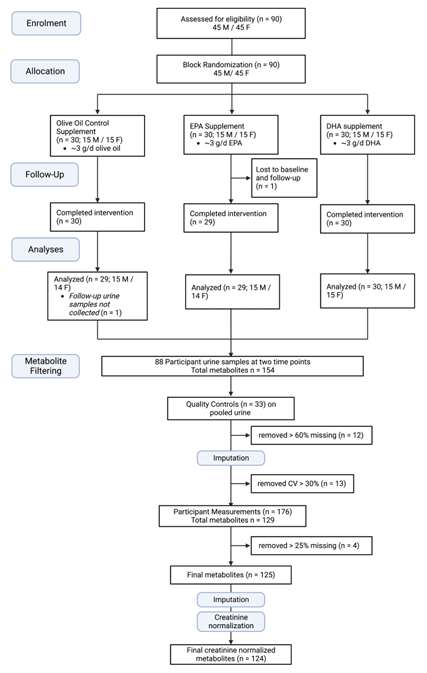
\includegraphics[width=0.8\linewidth]{../Figures/Participants_study_design} \caption{Flow diagram randomized controlled trial.}\label{fig:unnamed-chunk-1}
\end{figure}

\subsection{Baseline Participant Data Analysis in the Three Supplement
Groups}\label{baseline-participant-data-analysis-in-the-three-supplement-groups}

Group means for baseline participant data were calculated and are
reported in Table 1. There were no significant differences between the
three groups for baseline characteristics.

\begin{longtable}[]{@{}llll@{}}
\toprule\noalign{}
\textbf{Characteristics} & \textbf{OO} & \textbf{EPA} & \textbf{DHA} \\
\midrule\noalign{}
\endhead
\bottomrule\noalign{}
\endlastfoot
\emph{M/F,n} & 15/15 & 15/14 & 15/15 \\
\emph{Age,y} & 21.1 +/- 1.9 & 21.4 +/- 2.2 & 22.2 +/- 2.3 \\
\emph{Weight,kg} & 69.0 +/- 10.9 & 71.0 +/- 12.0 & 72.7 +/- 14.9 \\
\emph{BMI,kg/m2} & 24.1 +/- 3.5 & 23.1 +/- 2.8 & 23.7 +/- 3.4 \\
\end{longtable}

\subsection{Identification of Urinary Metabolites Associated with EPA
and/or DHA
Supplementation}\label{identification-of-urinary-metabolites-associated-with-epa-andor-dha-supplementation}

To avoid spurious results, we applied multiple statistical methods to
identify urinary metabolites associated with the O3I. These urinary
metabolites comprised 17 (out of 125) annotated unknown ions via
high-resolution MS tentatively identified using collision induced
dissociation MS/MS. First, we used supervised and unsupervised
clustering methods to obtain a general overview of the urine metabolome
data variance that distinguishes the supplement groups from one another.
Second, we used pairwise analyses to examine changes in
creatinine-normalized metabolite responses in relation to
supplementation and time. Finally, we investigated those urinary
metabolites that directly contributed to predicting variability in the
O3I. Collectively, these complimentary statistical approaches were used
to select and identify urinary metabolites that were consistently and
temporally associated with n3-LCPUFA status as compared to the OO
control.

\subsection{Distinguishing Supplementation Groups with Unsupervised and
Supervised Clustering
Approaches}\label{distinguishing-supplementation-groups-with-unsupervised-and-supervised-clustering-approaches}

First, we performed a global analysis to examine if urinary metabolite
profiles could distinguish between the three supplement groups from
baseline. Overall, the technical variance for repeated analysis of 125
metabolites (including creatinine) in a pooled urine sample was
acceptable with a median CV = 13.4\% for QCs (n = 33) as compared to
their greater between-subject biological variance with a median CV =
60.5\% (n = 178). Two-dimensional PCA plots of 124 creatinine-normalized
urinary metabolites at both baseline (Figure S1a) and 12 weeks (Figure
S1b) were unable to distinguish the three supplement groups from one
another. Furthermore, a PCA plot corresponding to the delta response
values (i.e., RPA after supplementation -- RPA at baseline) for urinary
metabolites was also unable to distinguish the three supplement groups
(Figure S1c), with the first two components (PC1 and PC2) only
explaining 20.4\% of the total variance in the dataset. Similarly, the
three supplement groups were not well distinguished by relative \%FA
(Figure S1d) or by quantitative FA data (Figure S1e). In all instances,
participants from all groups were clustered around the centre of each
plot with no clear distinction observed between groups. We next
performed supervised PLS-DA and sparse PLS-DA (sPLS-DA) to better
distinguish the three supplementation groups in this study (Figure 2).
While less total variation was explained by the first two principal
components (i.e., PC1 + PC2 = 14\% and 9\% for Figure 2a, b,
respectively) than in the PCA model, the visual separation between
groups was slightly improved. Since we hypothesized that only a small
subset of urinary metabolites would relate to changes in EPA and/or DHA
erythrocyte content, we next performed a sPLS-DA for urinary metabolite
biomarker selection.

\begin{figure}
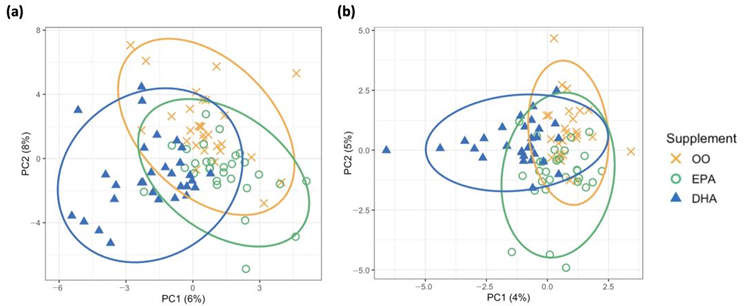
\includegraphics[width=0.8\linewidth]{../Figures/PC1_O3I} \caption{Participant plots of relative peak area (RPA) delta values for (a) 124 creatinine-normalized metabolite responses in PLS-DA and (b) 15 selected urinary metabolites for each principal component in sPLS-DA, coloured by group (OO = orange, EPA = green, DHA = blue).}\label{fig:unnamed-chunk-2}
\end{figure}

Variable selection via sPLS-DA identified the top-ranked 15 urinary
metabolites associated with OO, EPA, and DHA supplementation for both
PC1 and PC2 (Figure S2). The metabolites selected in PC1 were related to
DHA supplementation (blue), whereas those selected in PC2 largely
corresponded to metabolites related to EPA supplementation (green). The
top-ranked urinary metabolites having the largest weighting on PC1 were
an unknown divalent anion (221.075:0.927:n), as well as an unknown
cation (164.074:0.614:p) that was tentatively identified as
S-carboxypropylcysteamine (CPCA) based on annotation of their slower
positive mobility (at pH 1.8) due to a more acidic alpha-carboxylic acid
moiety, resulting in their longer apparent migration times (e.g.,
S-propylcysteine). Overall, urinary CPCA was measured consistently with
acceptable technical precision (CV = 9.8\%, n = 33) throughout the
study. The third and fourth most significant urinary metabolites
classified via sPLS-DA along PC1 were tetrahydroaldosterone glucuronide
and an unknown anion isomer (241.120:0.653:n), which was tentatively
identified as a dipeptide when using MS/MS in negative ion mode, namely
pyroglutamylisoleucine (pGlu-Ile) (Figure S4). As there were two
partially resolved isobars in the extracted ion electropherogram with
analogous MS/MS spectra, isobars were distinguished by their apparent
migration times, with the slower migrating isomer likely being
pyroglutamylleucine (pGlu-Leu). Overall, the urinary metabolites
contributing the most loading weight for PC1 (Figure S2a) were an
unknown dianion (221.075:0.927:n), CPCA (164.074:0.613:p),
tetrahydroaldosterone glucuronide, and pGlu-Ile. Top loading weights for
PC2 (Figure S2b) corresponded to choline, glucuronic acid, an unknown
dianion (88.004:1.622:n), and quinic acid. Structural elucidation of the
unknown dianion (221.075:0.927:n) was not feasible due to its low
abundance in urine that prevented the acquisition of an MS/MS spectra
(Figure S5). Its MS/MS spectrum at an optimal collisional energy under
positive ion mode (Figure 3) together with its co-migration after
spiking a standard of CPCA in pooled urine (Figure S3). Other isobaric
candidate ions having the same molecular formula (e.g., ethione,
N-methylmethionine, S-methylmethionine, etc.) were excluded as likely
candidates based.

\begin{figure}
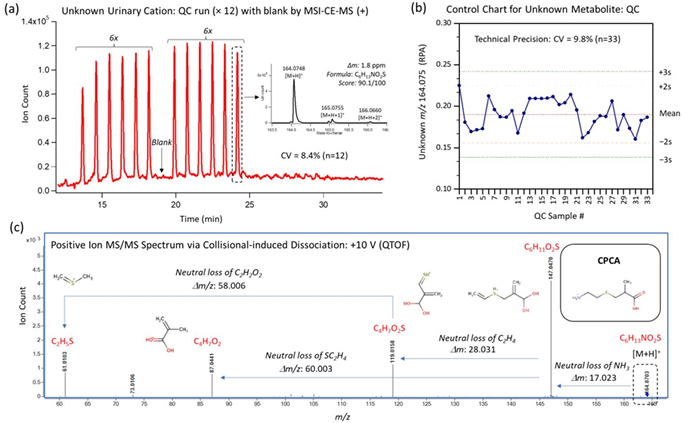
\includegraphics[width=0.8\linewidth]{../Figures/Chromatograms} \caption{Structural elucidation of S-carboxypropylcysteamine (CPCA).}\label{fig:unnamed-chunk-3}
\end{figure}

\subsection{Increases in Urinary CPCA Are Associated with n3-LCPUFA
Erythrocyte
Content}\label{increases-in-urinary-cpca-are-associated-with-n3-lcpufa-erythrocyte-content}

Finally, we performed additional analyses on the two lead urinary
biomarkers of the O3I (CPCA and the unknown dianion 221.075:0.927:n)
that were systematically identified in all three statistical approaches
(Table 3). Specifically, we examined whether the changes observed in
these urinary metabolites were specific to changes in the O3I through
measuring Pearson correlation coefficients ® with all other measured
erythrocyte fatty acids (Figure 6). Urinary CPCA was positively
correlated with the O3I (r = 0.30, p \textless{} 0.001) but also showed
correlations with both EPA (r = 0.19, p = 0.012) and DHA (r = 0.21, p =
0.004) individually. CPCA was also inversely correlated with AA (r =
0.30, p \textless{} 0.001) and myristic acid (r = 0.26, p \textless{}
0.001). However, CPCA was not correlated with any other measured fatty
acid. The unknown dianion (221.075:0.927:n) was more strongly correlated
with the O3I (r = 0.47, p \textless{} 0.001) and with DHA (r = 0.53, p
\textless{} 0.001) but was not correlated with EPA.

\begin{figure}
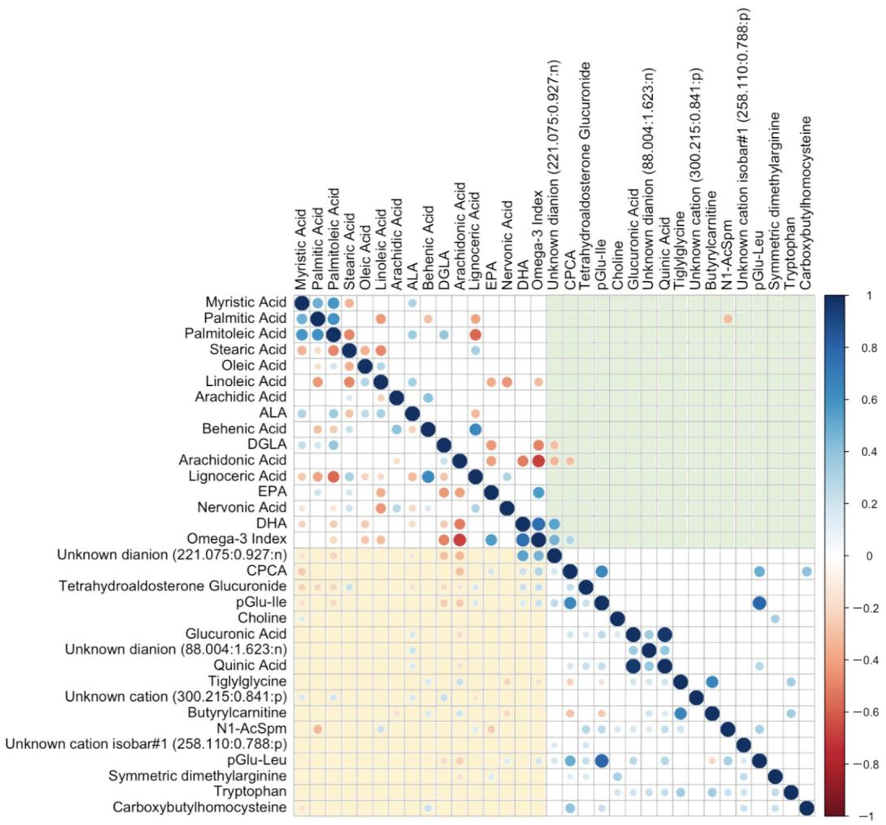
\includegraphics[width=0.8\linewidth]{../Figures/Most_relevant_metabolites} \caption{Correlation plot of relative \% fatty acids in erythrocytes and top 17 selected metabolites, where significant (p < 0.05 below diagonal, Padj < 0.05 above diagonal) correlations are indicated by sphere size (strength) and colour (blue = positive, red = negative).}\label{fig:unnamed-chunk-4}
\end{figure}

\section{Discussion}\label{discussion}

To the best of our knowledge, this study is the first to investigate
urinary metabolites as putative non-invasive biomarkers of the O3I using
a non-targeted metabolomics ap proach. Our results identified urinary
CPCA and an unknown dianion (221.075:0.927:n) as novel candidate urinary
biomarkers for O3I status in healthy, young individuals. While the
unknown dianion (221.075:0.927:n) was also identified as an indicator of
DHA sup plementation specifically, CPCA was found to be associated with
both EPA and DHA supplementation as compared to OO. More specifically,
both candidate urinary metabo lites were positively associated with the
O3I, and when compared to all 15 measured erythrocyte membrane-derived
phospholipid fatty acids, creatinine-normalized urinary CPCAlevels
showed specificity in their association with the O3I, whereas the
unknown dianion (221.075:0.927:n) showed a greater association with DHA.
As a supplement group classifier between EPA or DHA relative to OO,
urinary CPCA consistently outperformed other selected urinary
metabolites when using ROC curves (AUC \textgreater{} 80\%), whereas the
unknowndianion showed the highest performance specifically for DHA (AUC
\textgreater{} 90\%) with poor sensitivity for EPA. Similarly, both CPCA
(AUC = 73\%) and the unknown dianion (AUC=89\%)outperformed other
urinary metabolites when classifying a low (\textless4\%) versus high
(\textgreater8\%) O3I. Taken together, our robust analyses have
positioned urinary CPCA and the unknown dianion (221.075:0.927:n) as
novel surrogates for the O3I. Collectively, this work lays the
foundation for developing a convenient and non-invasive approach to
assess an individual's n3-LCPUFA status.

Urinary biomarkers represent an attractive option for nutrient
monitoring. Traditional dietary assessments estimate nutrient status,
but are limited in their ability to accurately capture variation in food
quality, intake, absorption, and metabolism {[}51{]}. Therefore,
biomarkers have the advantage of more accurately indicating the amount
of a nutrient available to tissues and organs. Current validated
nutrient biomarkers of n3-LCPUFA status such as the O3I {[}52{]} require
a small blood sample. Recently, Ly et al.~{[}53{]} reported two
phosphatidylcholine species can serve as circulating surrogate
biomarkers of the O3I directly in serum or plasma rather than hydrolyzed
EPA and DHA measured from the phospholipid fraction of erythrocyte
membranes. Yet, access to blood specimens may still represent a barrier
to their use at both the individual and population levels. In contrast,
the use of urinary metabolites as a proxy for the O3I could improve ease
of monitoring while capturing physiologically relevant information.
Although numerous reports in the literature have identified potential
candidate biomarkers of n3-LCPUFA status, very few have been validated
and are therefore currently of limited use. While a validation pipeline
for biomarkers of food intake and/or nutrient status has been proposed
{[}54{]}, meeting all criteria for establishing the biological validity
and analytical performance of a biomarker remains a challenge.
Nevertheless, the power of a validated urinary biomarker for nutrient
status has wide-scale implications for use in personalized health,
nutrition and epidemiological research, and clinical risk assessment for
cardiovascular events and hypertriglyceridemia, amongst others.

Through our analyses, we found that urinary CPCA was significantly
correlated with changes in the O3I and AA satisfying both a dose and
temporal response as criteria. Moreover, urinary CPCA was reliably
measured with acceptable technical precision (mean CV \textless{} 10\%)
with no missing values using a validated multiplexed separation platform
and data workflow for metabolomics based on MSI-CE-MS {[}29{]}. Also,
urinary CPCA increased consistently following both EPA and DHA
supplementation in our cohort of young Canadian adults having a low
average O3I status at baseline. Overall, no other putative urinary
biomarker associated with the O3I identified in our study had higher
sensitivity (89.6\% and 83.3\%) and specificity (72.4\% and 72.4\%) for
both EPA and DHA supplementation, respectively. We hypothesized that the
inverse relationship between CPCA and AA stems primarily from the known
reduction in AA membrane content observed with increased n3-LCPUFA
intake {[}1{]}. Indeed, we found that when the relative levels of
erythrocyte EPA and DHA increased, there were proportional reductions in
AA. In a dose--response randomized controlled trial examining EPA + DHA
supplementation in healthy male and female participants, Flock et al.
{[}52{]} reported that erythrocyte EPA and DHAcontent increased
concomitant with comparable reductions in AA content. Similarly, Vidgren
et al.~{[}55{]} showed significant reductions in erythrocyte AA content
in individuals consumingafishoilsupplementoreatingafishdiet.
Ourfindingsalignwiththeseprevious studies. Due to the close relationship
between n3-LCPUFA and AA erythrocyte membrane content, the specificity
of CPCA related to the O3I may falsely implicate the latter. Indeed,
there was an equivalent strength of association of urinary CPCA
inversely with AA and positively with the O3I (r = 0.30) as compared to
EPA or DHAalone. Nevertheless, increases in the O3I concomitant with
decreases in AA are generally indicative of good health {[}56{]}.

Urinary metabolites related to fish intake have been proposed as
potential urinary biomarkers in previous studies. In a cross-sectional
analysis of the INTERMAP study, Gibson et al.~{[}23{]} found TMAO and
taurine were capable of distinguishing between low and high fish intake
in a Japanese subpopulation. Our study identified and quantified urinary
TMAO, but we did not find that this metabolite was capable of
distinguishing betweenlowandhighO3Ilevels. Takentogether, thissuggests
that TMAOmaybeaurinary biomarker related to marine meat protein intake
rather than n3-LCPUFA. A randomized controlled trial in individuals with
type-2 diabetes supplemented with fish oil, flaxseed oil, or corn oil
showed significant increases in urinary CMPF in the fish oil group,
which was also highly correlated to serum CMPF {[}24{]}. The association
of urinary CMPF could not be evaluated in our study as it was not
detected via MSI-CE-MS. Therefore, both TMAO and CMPFrequire further
evaluation to clarify their use as biomarkers of fish/fish oil intake
versus n3-LCPUFA status.

To the best of our knowledge, only two previous studies have explored
associations between the O3I and urinary metabolites. Bigornia et al.
{[}22{]} reported an inverse rela tionship between the O3I and
depressive symptoms in older adults with obesity having high urinary
8-OHdG, i.e., a biomarker of oxidative stress. However, no association
was found between the O3I and urinary 8-OHdG at baseline and it was not
evaluated at the 2 yfollow-up, which suggest that this relationship
between depressive symptoms and the O3I may be indirectly related to
oxidative stress. In a separate cross-sectional study in young and
healthy adults, Filipovic et al.~{[}21{]} reported an inverse
relationship between the O3I and the albumin-to-creatine (ACR) ratio
after adjusting for various covariates, such as age, sex, BMI, and
smoking status. Neither 8-OHdG nor albumin were detected in our urinary
metabolomic analysis when using MSI-CE-MS, which prevents our
independent verification of the relationship between these metabolites
and the O3I in our study.

Currently, there are nine isobaric candidate metabolites in the HMDB
that match the most likely molecular formula for the urinary metabolite
we have tentatively identified as CPCA(164.074:0.613:p-C6H13NO2S). While
the unambiguous identification of CPCA is ongoing, we have ruled out
four isobaric ions based on migration behaviour and structural
properties that impact their ionization state (i.e., pKa) and
corresponding migration times. Of the remaining isobaric ion candidates
reported in the HMDB, the structural properties of CPCA's functional
groups best reflect the migration time and characterization shown in the
extracted ion electropherogram (Figure 3). Furthermore, additional
studies are necessary to clarify the underlying biochemical link(s)
between n3-LCPUFA and CPCA as well as establish reference intervals for
urinary CPCA in larger populations to define optimal cut-off
concentrations associated with the O3I.

Additionally, while demonstrating astrongassociation to theO3I,
anunknowndianion (221.075:0.927:n) showed specificity in its
relationship to DHA supplementation with seemingly little-to-no
association with EPA supplementation. In the absence of a confirmed
identification for this urinary metabolite, it is challenging to
speculate on the biochemical significance of this finding and its link
with DHA; however, this currently unidentified metabolite may prove to
be a specific marker of DHA in the body and thus warrants continued
investigation. Improved concentration sensitivity is needed to measure
this lower abundance hydrophilic urinary metabolite, which is also
needed when acquiring better quality MS/MS spectra.

Our study has several strengths. First, the participant samples used
were collected during a randomized placebo-controlled trial that
included matching baseline and 12-week fasted blood and first-void urine
samples. Second, erythrocyte fatty acid measurements were examined using
both relative \% and quantitative (ng FA/mg Hb) values, thus al lowing
for the robust verification of the relationship between erythrocyte EPA
and DHA with CPCA. All three statistical methods performed on all 124
creatinine-normalized urinary metabolites confirmed similar results,
where CPCA and an unknown dianion (221.075:0.927:n) were consistently
identified using several different approaches. Addi tionally, we
conducted an initial proof-of-principle study 2 years prior to the
present full study that first identified a relationship between CPCA and
high-dose DHA intake relative to OOwith goodmutual agreement and
reproducibility, thus demonstrating the stability of CPCAinfrozen urine
samples following repeat analysis after thawing and long-term storage.
Finally, to rule out potential metabolite contamination, we analyzed
both lipid and aqueous extracts of the OO, EPA, and DHA capsules and did
not detect CPCA, the unknown dianion (221.075:0.927:n), and other
polar/hydrophilic biomarker candidates reported in this work,
reinforcing that the changes in concentration of these endogenous
urinary metabolites reflect biochemical changes in study participants
following high-dose EPAand/or DHAintake.

There are also several limitations to our study. First, we acknowledge
the small and relatively homogenous sample size of the current study.
Indeed, participants were all young (18--30 y) and healthy individuals
that do not necessarily reflect variation seen in free-living
populations. Thus, the generalizability of urinary CPCA and the unknown
dianion (221.075:0.927:n) as non-invasive biomarkers for the O3I needs
to be confirmed in populations that vary in age, ethnicity, genetics,
and health status. Additionally, other lifestyle factors were not
accounted for during the clinical trial, such as physical activity,
alcohol consumption, and dietary patterns. Future studies will need to
measure macro- and micronutrient intakes to ensure that changes in
urinary metabolites are specific to changes in n3-LCPUFA intake.
Furthermore, first-void urine samples used in our metabolomics analyses
are more susceptible to acute or diurnal changes in urine composition,
which maydiminish the accuracy of associations drawn between urine
metabolites and long-term changes in erythrocyte fatty acid composition.
As such, 24 h urine samples and/or several repeat spot urine samples
collected over time from the same individual could provide a more
reliable metabolite assessment of O3I status and improve the strength of
associations between urinary metabolites and erythrocyte fatty acid
composition. Future work needs to explore the stability of these
metabolites in urine through comparing fasting first-void urine samples
with 24 h samples, as well as day-to-day variability. Moreover, urine
samples were analyzed on a single metabolomic platform (MSI-CE-MS),
which is well suited for identifying polar or ionic compounds since they
are predominantly excreted in human urine {[}57{]}. However, due to the
selectivity and sensitivity of liquid chromatography, gas
chromatography, and CE-MS techniques to capture different types of
compounds, the use of complementary instrumental platforms may uncover
additional urinary biomarkers of the O3I {[}58,59{]}. Ultimately, this
could lead to the identification of a larger panel of urinary
metabolites that may reflect changes in the O3I compared to CPCA and/or
the unknown dianion (221.075:0.927:n) alone while also independently
validating biomarker outcomes across platforms {[}60{]}. Furthermore, it
is unclear what minimum dosage of n3 LCPUFA is needed to elicit a
significant increase in these candidate urinary biomarkers above
endogenous background levels in human urine. Since participants in the
present trial received moderately high doses of EPA or DHA
(\textasciitilde3 g per day), future studies should consider different
doses and formulations of n3-LCPUFA supplementation. Finally, the
underlying biochemical connection between these candidate urinary
biomarkers and n3 LCPUFA remains to be elucidated.

\section{Conclusions}\label{conclusions}

We report the identification of a novel panel of urinary metabolites as
robust, non invasive biomarkers of n3-LCPUFA status. Specifically, our
findings reveal that urinary CPCAandanunknowndianion (221.075:0.927:n)
may serve as promising biomarkers for the O3I, and thereby lay the
groundwork for establishing an objective and non-invasive test for the
personalized assessment of n3-LCPUFA status. We anticipate that an
eventual non-invasive test could be used for early screening of health
risks and self-monitoring of the O3I following personalized dietary
changes. However, additional studies confirming the sensitivity and
specificity of these urinary metabolites as biomarkers of the O3I
require further validation prior to considering their clinical utility.

\section{References}\label{references}

\begin{enumerate}
\def\labelenumi{\arabic{enumi}.}
\tightlist
\item
  Calder, P.C. Omega-3 Fatty Acids and Inflammatory Processes. Nutrients
  2010, 2, 355--374. {[}CrossRef{]} {[}PubMed{]}
\item
  Mozaffarian, D.; Wu, J.H.Y. Omega-3 Fatty Acids and Cardiovascular
  Disease: Effects on Risk Factors, Molecular Pathways, and Clinical
  Events. J. Am. Coll. Cardiol. 2011, 58, 2047--2067. {[}CrossRef{]}
\item
  Abdelhamid, A.S.; Brown, T.J.; Brainard, J.S.; Biswas, P.; Thorpe,
  G.C.; Moore, H.J.; Deane, K.H.; Summerbell, C.D.; Worthington, H.V.;
  Song, F.; et al.~Omega-3 Fatty Acids for the Primary and Secondary
  Prevention of Cardiovascular Disease. Cochrane Database Syst. Rev.
  2020, 3, CD003177. {[}CrossRef{]} {[}PubMed{]}
\item
  Reimers, A.; Ljung, H. The Emerging Role of Omega-3 Fatty Acids as a
  Therapeutic Option in Neuropsychiatric Disorders. Ther. Adv.
  Psychopharmacol. 2019, 9, 204512531985890. {[}CrossRef{]}
\item
  Harris, W.S.; Tintle, N.L.; Imamura, F.; Qian, F.; Korat, A.V.A.;
  Marklund, M.; Djoussé, L.; Bassett, J.K.; Carmichael, P.H.; Chen,
  Y.Y.; et al.~Blood N-3 Fatty Acid Levels and Total and Cause-Specific
  Mortality from 17 Prospective Studies. Nat. Commun. 2021, 12, 2329.
  {[}CrossRef{]}
\item
  Burdge, G.C.; Wootton, S.A. Conversion of-Linolenic Acid to
  Eicosapentaenoic, Docosapentaenoic and Docosahexaenoic Acids in Young
  Women. Br. J. Nutr. 2002, 88, 411--420. {[}CrossRef{]} {[}PubMed{]}
\item
  Plourde, M.; Cunnane, S.C. Extremely Limited Synthesis of Long Chain
  Polyunsaturates in Adults: Implications for Their Dietary Essentiality
  and Use as Supplements. Appl. Physiol. Nutr. Metab. 2007, 32,
  619--634. {[}CrossRef{]} {[}PubMed{]}
\item
  Kipnis, V.; Midthune, D.; Freedman, L.; Bingham, S.; Day, N.E.;
  Riboli, E.; Ferrari, P.; Carroll, R.J. Bias in Dietary-Report
  Instruments and Its Implications for Nutritional Epidemiology. Public
  Health Nutr. 2002, 5, 915--923. {[}CrossRef{]}
\item
  Poslusna, K.; Ruprich, J.; De Vries, J.H.M.; Jakubikova, M.; Van'T
  Veer, P. Misreporting of Energy and Micronutrient Intake Estimated by
  Food Records and 24hour Recalls, Control and Adjustment Methods in
  Practice. Br. J. Nutr. 2009, 101, S73--S85. {[}CrossRef{]}
\item
  vonSchacky, C. Omega-3 Index and Cardiovascular Health. Nutrients
  2014, 6, 799--814. {[}CrossRef{]}
\item
  Cholewski, M.; Tomczykowa, M.; Tomczyk, M. A Comprehensive Review of
  Chemistry, Sources and Bioavailability of Omega-3 Fatty Acids.
  Nutrients 2018, 10, 1662. {[}CrossRef{]} {[}PubMed{]}
\item
  Tu, W.C.; Mühlhäusler, B.S.; Yelland, L.N.; Gibson, R.A. Correlations
  between Blood and Tissue Omega-3 LCPUFA Status Following Dietary ALA
  Intervention in Rats. Prostaglandins Leukot. Essent. Fat. Acids 2013,
  88, 53--60. {[}CrossRef{]} {[}PubMed{]}
\item
  Harris, W.S.; Von Schacky, C. The Omega-3 Index: A New Risk Factor for
  Death from Coronary Heart Disease? Prev. Med. 2004, 39, 212--220.
  {[}CrossRef{]} {[}PubMed{]}
\item
  McLenon, J.; Rogers, M.A.M. The Fear of Needles: A Systematic Review
  and Meta-Analysis. J. Adv. Nurs. 2019, 75, 30--42. {[}CrossRef{]}
\item
  Mcmurtry, C.M.; Taddio, A.; Noel, M.; Antony, M.M.; Rieder, M.J.;
  Robson, K.; Uleryk, E.; Votta, E. Exposure-Based Interventions for the
  Management of Individuals with High Levels of Needle Fear across the
  Lifespan: A Clinical Practice Guideline and Call for Further Research.
  Cogn. Behav. Ther. 2016, 45, 217--235. {[}CrossRef{]}
\item
  Dempsey, M.; Rockwell, M.S.; Wentz, L.M. The Influence of Dietary and
  Supplemental Omega-3 Fatty Acids on the Omega-3 Index: A Scoping
  Review. Front. Nutr. 2023, 10, 1072653. {[}CrossRef{]}
\item
  Rafiq, T.; Azab, S.M.; Teo, K.K.; Thabane, L.; Anand, S.S.; Morrison,
  K.M.; De Souza, R.J.; Britz-Mckibbin, P. Nutritional Metabolomics and
  the Classification of Dietary Biomarker Candidates: A Critical Review.
  Adv. Nutr. 2021, 12, 2333--2357. {[}CrossRef{]}
\item
  O'Gorman, A.; Brennan, L. The Role of Metabolomics in Determination of
  New Dietary Biomarkers. Proc. Nutr. Soc. 2017, 76, 295--302.
  {[}CrossRef{]}
\item
  Gao,Q.; Praticò, G.; Scalbert, A.; Vergères, G.; Kolehmainen, M.;
  Manach, C.; Brennan, L.; Afman, L.A.; Wishart, D.S.; Andres Lacueva,
  C.; et al.~A Scheme for a Flexible Classification of Dietary and
  Health Biomarkers. Genes Nutr. 2017, 12, 1--15. {[}CrossRef{]}
\item
  Clarke, E.D.; Rollo, M.E.; Collins, C.E.; Haslam, R.L.; Pezdirc, K.
  Urinary Biomarkers of Dietary Intake: A Review. Nutr. Rev.~2020, 78,
  364--381. {[}CrossRef{]}
\item
  Filipovic, M.G.; Reiner, M.F.; Rittirsch, S.; Irincheeva, I.;
  Aeschbacher, S.; Grossmann, K.; Risch, M.; Risch, L.; Limacher, A.;
  Conen, D.; et al.~Blood Omega-3 Fatty Acids Are Inversely Associated
  With Albumin-Creatinine Ratio in Young and Healthy Adults (The
  Omega-Kid Study). Front. Cardiovasc. Med. 2021, 8, 622619.
  {[}CrossRef{]}
\item
  Bigornia, S.J.; Harris, W.S.; Falcón, L.M.; Ordovás, J.M.; Lai, C.Q.;
  Tucker, K.L. The Omega-3 Index Is Inversely Associated with Depressive
  Symptoms among Individuals with Elevated Oxidative Stress Biomarkers.
  J. Nutr. 2016, 146, 758--766. {[}CrossRef{]} {[}PubMed{]}
\item
  Gibson, R.; Lau, C.H.E.; Loo, R.L.; Ebbels, T.M.D.; Chekmeneva, E.;
  Dyer, A.R.; Miura, K.; Ueshima, H.; Zhao, L.; Daviglus, M.L.; et al.
  The Association of Fish Consumption and Its Urinary Metabolites with
  Cardiovascular Risk Factors: The International Study of
  Macro-/Micronutrients and Blood Pressure (INTERMAP). Am. J. Clin.
  Nutr. 2020, 111, 280--290. {[}CrossRef{]}
\item
  Ruan,Y.; Zheng, J.; Ren, Y.; Tang, J.; Li, J.; Li, D. Changes of Urine
  Metabolites in Response to N-3 Fatty Acid Supplements and Their
  Correlation with Metabolic Risk Factors in Patients with Type 2
  Diabetes. Food Funct. 2019, 10, 2471--2479. {[}CrossRef{]}
\item
  Lee, J.B.; Notay, K.; Klingel, S.L.; Chabowski, A.; Mutch, D.M.;
  Millar, P.J. Docosahexaenoic Acid Reduces Resting Blood Pressure but
  Increases Muscle Sympathetic Outflow Compared with Eicosapentaenoic
  Acid in Healthy Men and Women. Am. J. Physiol. Hear. Circ. Physiol.
  2019, 316, H873--H881. {[}CrossRef{]}
\item
  Metherel, A.H.; Irfan, M.; Klingel, S.L.; Mutch, D.M.; Bazinet, R.P.
  Compound-Specific Isotope Analysis Reveals No Retroconver sion of DHA
  to EPAbut Substantial Conversion of EPA to DHA Following
  Supplementation: A Randomized Control Trial. Am. J. Clin. Nutr. 2019,
  110, 823--831. {[}CrossRef{]} {[}PubMed{]}
\item
  Folch, J.; Lees, M.; Sloane Stanley, G.H. A Simple Method for the
  Isolation and Purification of Total Lipides from Animal Tissues. J.
  Biol. Chem. 1957, 226, 497--509. {[}CrossRef{]} {[}PubMed{]}
\item
  Mcglory, C.; Gorissen, S.H.M.; Kamal, M.; Bahniwal, R.; Hector, A.J.;
  Baker, S.K.; Chabowski, A.; Phillips, S.M. Omega-3 Fatty Acid
  Supplementation Attenuates Skeletal Muscle Disuse Atrophy during Two
  Weeks of Unilateral Leg Immobilization in Healthy Young Women. FASEB
  J. 2019, 33, 4586--4597. {[}CrossRef{]}
\item
  Shanmuganathan, M.; Kroezen, Z.; Gill, B.; Azab, S.; de Souza, R.J.;
  Teo, K.K.; Atkinson, S.; Subbarao, P.; Desai, D.; Anand, S.S.; et
  al.~The Maternal Serum Metabolome by Multisegment Injection-Capillary
  Electrophoresis-Mass Spectrometry: A High Throughput Platform and
  Standardized Data Workflow for Large-Scale Epidemiological Studies.
  Nat. Protoc. 2021, 16, 1966--1994. {[}CrossRef{]} {[}PubMed{]}
\item
  Yamamoto, M.; Pinto-Sanchez, M.I.; Bercik, P.; Britz-McKibbin, P.
  Metabolomics Reveals Elevated Urinary Excretion of Collagen
  Degradation and Epithelial Cell Turnover Products in Irritable Bowel
  Syndrome Patients. Metabolomics 2019, 15, 82. {[}CrossRef{]}
\item
  Yamamoto, M.; Shanmuganathan, M.; Hart, L.; Pai, N.; Britz-Mckibbin,
  P. Urinary Metabolites Enable Differential Diagnosis and Therapeutic
  Monitoring of Pediatric Inflammatory Bowel Disease. Metabolites 2021,
  11, 245. {[}CrossRef{]}
\item
  Nori de Macedo, A.; Mathiaparanam, S.; Brick, L.; Keenan, K.; Gonska,
  T.; Pedder, L.; Hill, S.; Britz-McKibbin, P. The Sweat Metabolome of
  Screen-Positive Cystic Fibrosis Infants: Revealing Mechanisms beyond
  Impaired Chloride Transport. ACS Cent. Sci. 2017, 3, 904--913.
  {[}CrossRef{]} {[}PubMed{]}
\item
  Wishart, D.S.; Guo, A.C.; Oler, E.; Wang, F.; Anjum, A.; Peters, H.;
  Dizon, R.; Sayeeda, Z.; Tian, S.; Lee, B.L.; et al.~HMDB 5.0: The
  HumanMetabolome Database for 2022. Nucleic Acids Res. 2022, 50,
  D622--D631. {[}CrossRef{]} {[}PubMed{]}
\item
  Wang,F.; Allen, D.; Tian, S.; Oler, E.; Gautam, V.; Greiner, R.; Metz,
  T.O.; Wishart, D.S. CFM-ID 4.0---A Web Server for Accurate MS-Based
  Metabolite Identification. Nucleic Acids Res. 2022, 50, W165--W174.
  {[}CrossRef{]} {[}PubMed{]}
\item
  DiBattista, A.; McIntosh, N.; Lamoureux, M.; Al-Dirbashi, O.Y.;
  Chakraborty, P.; Britz-McKibbin, P. Temporal Signal Pattern
  Recognition in Mass Spectrometry: A Method for Rapid Identification
  and Accurate Quantification of Biomarkers for Inborn Errors of
  Metabolism with Quality Assurance. Anal. Chem. 2017, 89, 8112--8121.
  {[}CrossRef{]} {[}PubMed{]}
\item
  Saoi, M.; Li, A.; McGlory, C.; Stokes, T.; von Allmen, M.T.; Phillips,
  S.M.; Britz-Mckibbin, P. Metabolic Perturbations from Step Reduction
  in Older Persons at Risk for Sarcopenia: Plasma Biomarkers of Abrupt
  Changes in Physical Activity. Metabolites 2019, 9, 134. {[}CrossRef{]}
  {[}PubMed{]}
\item
  Pluskal, T.; Castillo, S.; Villar-Briones, A.; Orešiˇ c, M. MZmine 2:
  Modular Framework for Processing, Visualizing, and Analyzing Mass
  Spectrometry-Based Molecular Profile Data. BMC Bioinform. 2010, 11,
  395. {[}CrossRef{]}
\item
  RCore Team. R: A Language and Environment for Statistical Computing; R
  Foundation for Statistical Computing: Vienna, Aus tria, 2020.
\item
  Posit Team. RStudio: Integrated Development Environment for R. Posit
  Software; PBC: Boston, MA, USA, 2020.
\item
  Kassambara, A.; Mundt, F. Factoextra: Extract and Visualize the
  Results of Multivariate Data Analyses; R Package Version 1.0.7.
\item
  Available online: \url{https://CRAN.R-project.org/package=factoextra}
  (accessed on 9 September 2022).
\item
  Rohart,F.; Gautier, B.; Singh, A.; Lê Cao, K.A. MixOmics: An R Package
  for 'omics Feature Selection and Multiple Data Integration. PLoS
  Comput. Biol. 2017, 13, e1005752. {[}CrossRef{]}
\item
  Kassambara, A. rstatix: Pipe-Friendly Framework for Basic Statistical
  Tests; R Package Version 1.4.8. 2022. Available online:
  \url{https://CRAN.R-project.org/package=rstatix} (accessed on 22
  November 2022).
\item
  Pinheiro, J.; Bates, D.; R Core Team. nlme: Linear and Nonlinear Mixed
  Effects Models; R Package Version 3.1-157. 2022. Available online:
  \url{https://CRAN.R-project.org/package=nlme} (accessed on 9 September
  2022).
\item
  Lenth, R.V. Emmeans: Estimated Marginal Means, Aka Least-Squares
  Means; R Package Version 1.4.8. 2022. Available online:
  \url{https://CRAN.R-project.org/package=emmeans} (accessed on 9
  September 2022).
\item
  Groll, A. GlmmLasso: Variable Selection for Generalized Linear Mixed
  Models by L1-Penalized Estimation; R Package Version 1.6.2. 2022.
  Available online: \url{https://CRAN.R-project.org/package=glmmLasso}
  (accessed on 9 September 2022).
\item
  Robin, X.; Turck, N.; Hainard, A.; Tiberti, N.; Lisacek, F.; Sanchez,
  J.-C.; Mueller, M. PROC: An Open-Source Package for R and S+ to
  Analyze and Compare ROC Curves. BMC Bioinform. 2011, 8, 12--77.
  {[}CrossRef{]}
\item
  Wickham, H.ggplot2: Elegant Graphics for Data Analysis. Springer: New
  York, NY, USA, 2016; ISBN 978-3-319-24277-4.
\item
  Wei, T.; Simko, V. R package `corrplot': Visualization of a
  Correlation Matrix. R Package Version 0.92. 2021. Available online:
  \url{https://github.com/taiyun/corrplot} (accessed on 9 September
  2022).
\item
  Revelle, W. psych: Procedures for Psychological, Psychometric, and
  Personality Research; R Package Version 2.3.9. 2022. Available online:
  \url{https://CRAN.R-project.org/package=psych} (accessed on 9
  September 2022).
\item
  Klingel, S.L.; Metherel, A.H.; Irfan, M.; Rajna, A.; Chabowski, A.;
  Bazinet, R.P.; Mutch, D.M. EPA and DHA Have Divergent Effects on Serum
  Triglycerides and Lipogenesis, but Similar Effects on Lipoprotein
  Lipase Activity: A Randomized Controlled Trial. Am. J. Clin. Nutr.
  2019, 110, 1502--1509. {[}CrossRef{]} {[}PubMed{]} Potischman, N.
  Biomarkers of Nutritional Exposure and Nutritional Status Biologic and
  Methodologic Issues for Nutritional Biomarkers 1. J. Nutr. 2003, 133,
  875S--880S. {[}CrossRef{]} {[}PubMed{]}
\item
  Flock, M.R.; Skulas-Ray, A.C.; Harris, W.S.; Etherton, T.D.; Fleming,
  J.A.; Kris-Etherton, P.M. Determinants of Erythrocyte Omega-3 Fatty
  Acid Content in Response to Fish Oil Supplementation: A Dose-Response
  Randomized Controlled Trial. J. Am. Heart Assoc. 2013, 2, 20--23.
  {[}CrossRef{]} {[}PubMed{]}
\item
  Ly, R.; MacIntyre, B.C.; Philips, S.M.; McGlory, C.; Mutch, D.M.;
  Britz-McKibbin, P. Lipidomic Studies Reveal Specific Circulating
  Phosphatidylcholines as Surrogate Biomarkers of Omega-3 Index. J.
  Lipid Res. 2023, 100445. {[}CrossRef{]} {[}PubMed{]}
\item
  Dragsted, L.O.; Gao, Q.; Scalbert, A.; Vergères, G.; Kolehmainen, M.;
  Manach, C.; Brennan, L.; Afman, L.A.; Wishart, D.S.; Andres Lacueva,
  C.; et al.~Validation of Biomarkers of Food Intake-Critical Assessment
  of Candidate Biomarkers. Genes Nutr. 2018, 13, 14. {[}CrossRef{]}
  {[}PubMed{]}
\item
  Vidgren, H.M.; Ågren, J.J.; Schwab, U.; Rissanen, T.; Hänninen, O.;
  Uusitupa, M.I.J. Incorporation of N-3 Fatty Acids into Plasma Lipid
  Fractions, and Erythrocyte Membranes and Platelets during Dietary
  Supplementation with Fish, Fish Oil, and Docosahexaenoic Acid-Rich Oil
  among Healthy Young Men. Lipids 1997, 32, 697--705. {[}CrossRef{]}
  {[}PubMed{]}
\item
  Simopoulos, A.P. The Importance of the Ratio of Omega-6/Omega-3
  Essential Fatty Acids. Biomed. Pharmacother. 2002, 56, 365--379.
  {[}CrossRef{]}
\item
  Bouatra, S.; Aziat, F.; Mandal, R.; Guo, A.C.; Wilson, M.R.; Knox, C.;
  Bjorndahl, T.C.; Krishnamurthy, R.; Saleem, F.; Liu, P.; et al. The
  HumanUrine Metabolome. PLoS ONE 2013, 8, e73076. {[}CrossRef{]}
\item
  Zeki, Ö.C.; Eylem, C.C.; Reçber, T.; Kır, S.; Nemutlu, E. Integration
  of GC--MS and LC--MS for Untargeted Metabolomics Profiling. J. Pharm.
  Biomed. Anal. 2020, 190, 113509. {[}CrossRef{]}
\item
  Dunn,W.B.;Ellis, D.I. Metabolomics: Current Analytical Platforms and
  Methodologies. TrAC Trends Anal. Chem. 2005, 24, 285--294.
  {[}CrossRef{]}
\item
  Shanmuganathan, M.; Sarfaraz, M.O.; Kroezen, Z.; Philbrick, H.; Poon,
  R.; Don-Wauchope, A.; Puglia, M.; Wishart, D.; Britz McKibbin, P. A
  Cross-Platform Metabolomics Comparison Identifies Serum Metabolite
  Signatures of Liver Fibrosis Progression in Chronic Hepatitis C
  Patients. Front. Mol. Biosci. 2021, 8, 676349. {[}CrossRef{]}
\end{enumerate}
\end{document}
